\documentclass[11pt]{article}
\usepackage[margin=1in]{geometry}
\usepackage[T1]{fontenc}
\usepackage[utf8]{inputenc}
\usepackage{amsmath,amssymb,amsthm,mathtools}
\usepackage{graphicx}
\usepackage{xcolor}
\usepackage{microtype}
\usepackage{enumitem}
\usepackage{tikz}
\usepackage[colorlinks=true,linkcolor=blue!55!black,citecolor=blue!55!black,urlcolor=blue!55!black]{hyperref}

\newtheorem{theorem}{Theorem}
\newtheorem{lemma}{Lemma}
\newcommand{\R}{\mathbb{R}}
\newcommand{\distI}{d_I}
\newcommand{\slope}{\mathsf{s}}
\newcommand{\setdist}{D}

\title{Singleton intrinsic-distance tests do not characterize compact eikonal spaces}
\author{Candidate counterexample packet for arXiv:2605.20486, Question 1}
\date{11 August 2026}

\begin{document}
\maketitle

\begin{center}
\fbox{\parbox{0.91\textwidth}{\textbf{Status: candidate counterexample, likely valid, subject to human review.}
The construction below gives a full negative answer to Question 1 of Salas, Tapia-Garc\'ia, and Venegas M.}}
\end{center}

\section{Source question}

The source is David Salas, Sebasti\'an Tapia-Garc\'ia, and Francisco Venegas M.,
\emph{The reach and limits of slope eikonal equations in compact spaces},
arXiv:2605.20486v1 [math.FA], submitted 19 May 2026 \cite{source}.
For a metric space $(X,d)$, its intrinsic distance is denoted by $d_I$, and the
descent slope of a real-valued function $f$ is
\[
  \slope[f](x)=\limsup_{y\to x}
  \frac{[f(x)-f(y)]_+}{d(x,y)}.
\]
Question 1 on printed page 25 asks:

\begin{quote}
Let $(X,d)$ be a compact metric space such that $d_I(\cdot,x)$ has slope $1$
on $X\setminus\{x\}$ for every $x\in X$. Is $(X,d)$ an eikonal space?
\end{quote}

The source proves that a compact metric space is eikonal if and only if
$\slope[d_I(\cdot,K)]=1$ on $X\setminus K$ for every nonempty closed $K$.
It also notes that it is enough to test closed countable $K$. Thus a negative
answer follows from a compact space on which every singleton test passes but
one closed countable-set test fails.

\section{Proof intuition}

The obstruction is a failure of uniformity in the endpoint. Attach countably
many polygonal arcs to a common root and let them accumulate on one straight
limit arc. Every finite arc makes a tiny dogleg near the root and then runs
almost parallel to the limit arc. For any \emph{fixed} target point, the
intrinsic-distance function only sees ordinary straight local geometry, so
its descent slope is one. The dogleg is at a fixed positive scale for that
fixed branch and disappears when the local-slope limit is taken.

Now put all branch endpoints into one closed set. At the root, the closest
endpoint is the endpoint of the limit arc. At the post-dogleg point of branch
$n$, the closest endpoint switches to the endpoint of branch $n$. This
switching makes the closed-set distance fall twice as fast as the ambient
Euclidean distance. The nearest endpoint varies with $n$, which is precisely
what no individual singleton test detects.

\begin{figure}[ht]
\centering
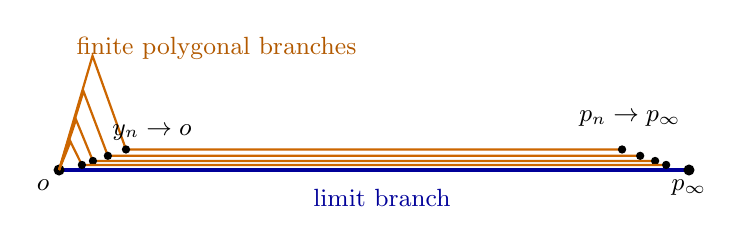
\begin{tikzpicture}[scale=1.0, every node/.style={font=\small}]
  \coordinate (o) at (0,0);
  \coordinate (pinf) at (8,0);
  \draw[very thick,blue!60!black] (o)--(pinf);
  \fill (o) circle (2pt) node[below left] {$o$};
  \fill (pinf) circle (2pt) node[below] {$p_\infty$};
  \foreach \h/\e/\lab in {1.45/0.85/1,1.00/0.62/2,0.64/0.43/3,0.36/0.29/4} {
    \coordinate (a) at (\e/2,\h);
    \coordinate (y) at (\e,0.18*\h);
    \coordinate (p) at (8-\e,0.18*\h);
    \draw[thick,orange!80!black] (o)--(a)--(y)--(p);
    \fill (y) circle (1.5pt);
    \fill (p) circle (1.5pt);
  }
  \node[orange!70!black] at (2.0,1.55) {finite polygonal branches};
  \node[blue!60!black,below] at (4.1,-0.12) {limit branch};
  \node at (7.25,0.65) {$p_n\to p_\infty$};
  \node at (1.18,0.48) {$y_n\to o$};
\end{tikzpicture}
\caption{Schematic planar projection. In the actual construction, different
finite branches lie in different half-planes in $\R^3$ and intersect only at
the root.}
\end{figure}

\section{Formal counterexample}

Write $\R^3=\R\times\R^2$. Let $o=(0,0)$ and
$p_\infty=(1,0)$. Choose pairwise non-collinear unit vectors
$v_n\in\R^2$, and set
\[
  \varepsilon_n=2^{-n-3},\qquad h_n=\varepsilon_n^2,
\]
\[
  a_n=\left(\frac{\varepsilon_n}{2},\varepsilon_n v_n\right),
  y_n=(\varepsilon_n,h_n v_n),
  p_n=(1-\varepsilon_n,h_n v_n).
\]
Define the straight limit arc and the finite polygonal arcs by
\[
  \Gamma_\infty=[o,p_\infty],\qquad
  \Gamma_n=[o,a_n]\cup[a_n,y_n]\cup[y_n,p_n],
\]
and let
\[
  X=\Gamma_\infty\cup\bigcup_{n\geq1}\Gamma_n
\]
with the metric $d$ induced by the Euclidean norm of $\R^3$.

The vectors may be chosen, for example, as
$v_n=(\cos(1/(n+1)),\sin(1/(n+1)))$. Distinct finite arcs then lie in
distinct half-planes through the first coordinate axis, and
$\Gamma_n\cap\Gamma_m=\{o\}$ for $n\ne m$, including $m=\infty$.

Let
\[
  \alpha_n=\operatorname{len}([o,a_n]\cup[a_n,y_n]).
\]
A direct computation gives
\begin{equation}\label{eq:alpha}
 \alpha_n=\varepsilon_n\left(
  \frac{\sqrt5}{2}+
  \sqrt{\frac14+(1-\varepsilon_n)^2}\right)>2\varepsilon_n.
\end{equation}
Indeed, $\varepsilon_n\leq1/16$, and the parenthesis is at least
$\sqrt5/2+17/16>2$. Hence the total length of $\Gamma_n$ is
\begin{equation}\label{eq:Ln}
  L_n=\alpha_n+(1-2\varepsilon_n)>1.
\end{equation}

\begin{lemma}\label{lem:tree}
$X$ is compact. Its intrinsic metric is the arclength tree metric on the arcs:
each finite branch can be left only through $o$, and the intrinsic distance
between two points is the length of the unique branch path joining them.
\end{lemma}

\begin{proof}
Take any sequence in $X$. A subsequence lying in a fixed compact polygonal
arc converges. Otherwise its branch indices tend to infinity. Points on the
two dogleg segments then converge to $o$, because their Euclidean norms are
$O(\varepsilon_n)$. Points on the horizontal tails have a subsequence whose
first coordinates converge to some $t\in[0,1]$, while their transverse
coordinates have norm $h_n\to0$; they converge to $(t,0)\in\Gamma_\infty$.
Thus $X$ is sequentially compact, hence compact.

For fixed $n$, every point of $\Gamma_n\setminus\{o\}$ has positive distance
from the other branches. Therefore $\Gamma_n\setminus\{o\}$ is relatively
open in $X\setminus\{o\}$, and a continuous path leaving $\Gamma_n$ must pass
through $o$. Since different branches meet only at $o$, their intrinsic
metric is exactly the asserted arclength tree metric.
\end{proof}

For a point $z$ on a finite branch, write $\sigma(z)=d_I(o,z)$ for its depth.
On the tail $[y_n,p_n]$, if $z=(t,h_n v_n)$, then
\begin{equation}\label{eq:depth-tail}
  \sigma(z)=\alpha_n+(t-\varepsilon_n)=t+c_n,
  \qquad c_n:=\alpha_n-\varepsilon_n>0.
\end{equation}

\begin{theorem}\label{thm:counterexample}
For every $p\in X$,
\[
  \slope[d_I(\cdot,p)](q)=1\qquad(q\in X\setminus\{p\}).
\]
Nevertheless, $X$ is not an eikonal space. More precisely, the closed
countable set
\[
  K=\{p_\infty\}\cup\{p_n:n\geq1\}
\]
satisfies
\[
  \slope[d_I(\cdot,K)](o)\geq2.
\]
Consequently Question 1 of arXiv:2605.20486 has a negative answer.
\end{theorem}

\begin{proof}
Fix $p\in X$ and put $F_p=d_I(\cdot,p)$.

\emph{Finite branches.}
Let $q\in\Gamma_n\setminus\{o,p\}$. A sufficiently small neighborhood of
$q$ lies in $\Gamma_n$. In the arclength coordinate $\sigma$, the function
$F_p$ is either $C+\sigma$ or $|\sigma-\sigma(p)|$. On each straight segment
incident to $q$, Euclidean distance from $q$ equals arclength. Thus every
descent quotient is at most one, and the incident segment pointing toward
$p$ along the tree realizes quotient one. This remains true at the two
polygonal vertices and at the endpoint of the branch.

\emph{The root.}
If $p$ lies on a finite branch, only points moving into that fixed branch can
decrease $F_p$ near $o$; its first segment is straight, so the quotient is
one. All other branches increase the distance to $p$. If $p$ lies on the
limit branch, its straight segment gives the same conclusion. Hence
$\slope[F_p](o)=1$ whenever $p\ne o$.

\emph{The limit branch.}
Let $q=(t,0)$ with $t>0$. Besides points of $\Gamma_\infty$, a sequence
approaching $q$ must eventually consist of tail points
$z_n=(r_n,h_n v_n)$ with $r_n\to t$ and branch indices tending to infinity.
By \eqref{eq:depth-tail}, $\sigma(z_n)=r_n+c_n$ with $c_n>0$.

If $p$ lies on a fixed finite branch at depth $b$, then eventually
\[
 [F_p(q)-F_p(z_n)]_+
 =[t-r_n-c_n]_+
 \leq[t-r_n]_+
 \leq d(q,z_n).
\]
If $p=(b,0)$ lies on the limit branch and $t\leq b$, then
$F_p(z_n)>F_p(q)$, so there is no descent. If $t>b$, then
\[
 [F_p(q)-F_p(z_n)]_+
 =[t-r_n-c_n-2b]_+
 \leq[t-r_n]_+
 \leq d(q,z_n).
\]
Thus cross-branch sequences never give slope larger than one. Moving along
the straight limit branch toward $p$ (or toward $o$ when $p$ is on a finite
branch) realizes quotient one. This completes the singleton-slope proof.

It remains to show failure for a closed set. Compactness and
$p_n\to p_\infty$ show that $K$ is closed. Equations \eqref{eq:Ln} and the
unit length of $\Gamma_\infty$ give
\[
  d_I(o,K)=1.
\]
At $y_n$, the closest point of $K$ is $p_n$, reached along the straight tail:
\[
  d_I(y_n,K)=d_I(y_n,p_n)=1-2\varepsilon_n.
\]
Indeed, every route from $y_n$ to any other point of $K$ first passes through
$o$ and has length greater than one. Finally,
\[
 \frac{d_I(o,K)-d_I(y_n,K)}{d(o,y_n)}
 =\frac{2\varepsilon_n}
 {\sqrt{\varepsilon_n^2+\varepsilon_n^4}}
 =\frac{2}{\sqrt{1+\varepsilon_n^2}}
 \longrightarrow2.
\]
Therefore $\slope[d_I(\cdot,K)](o)\geq2$, whereas the eikonal-space
characterization in the source requires this slope to equal one. Hence $X$
is not eikonal, despite passing every singleton test.
\end{proof}

\section{Verification and limitations}

The proof has no computational dependency. The bundled checker recomputes
\eqref{eq:alpha}, verifies $\alpha_n>2\varepsilon_n$ and $L_n>1$ over a large
finite range, and confirms convergence of the closed-set descent quotient to
two. The formal proof, rather than the finite check, establishes the result
for every $n$.

The conclusion concerns exactly the compact singleton-test question. It does
not classify noncompact eikonal spaces or other Hamilton-Jacobi equations.
The counterexample is a compact subset of Euclidean three-space with its
induced metric; its intrinsic metric is non-geodesically compatible with the
ambient chord metric at a sequence of shrinking doglegs.

\section{Novelty check and review recommendation}

On 11 August 2026, the run indexes were searched for arXiv:2605.20486 and for
the phrases ``slope eikonal'', ``singleton intrinsic distance'', and close
variants. Bounded primary arXiv searches for the exact question, title, and
singleton formulation found only source version v1 and no later answer. The
source arXiv record still lists only v1. Novelty confidence is therefore
moderate to high, with the usual caveat that a two-month-old problem may have
unindexed private or forthcoming work.

Human review should focus on two points: (i) the assertion that a finite
branch can be left only through the root, which identifies the intrinsic tree
metric; and (ii) the cross-branch slope estimate on the limit arc. Both are
spelled out explicitly above and are independent of computation.

\appendix
\section{Source-page evidence}

Figure~\ref{fig:source} reproduces printed page 25 of the source PDF, including
the exact open question.

\begin{figure}[p]
\centering

\includegraphics[height=0.88\textheight]{figures/open_problem_crop.png}
\caption{Source paper, printed page 25: the singleton-test conjecture and
Question 1.}\label{fig:source}
\end{figure}

\begin{thebibliography}{9}
\bibitem{source}
D. Salas, S. Tapia-Garc\'ia, and F. Venegas M.,
\emph{The reach and limits of slope eikonal equations in compact spaces},
arXiv:2605.20486v1 [math.FA], 2026.
\end{thebibliography}

\end{document}

